% --------------------------------------------------------------
% This is all preamble stuff that you don't have to worry about.
% Head down to where it says "Start here"
% --------------------------------------------------------------
 
\documentclass[12pt]{article}
 
\usepackage[margin=1in]{geometry} 
\usepackage{amsmath,amsthm,amssymb}
\usepackage{graphicx}

\newcommand{\N}{\mathbb{N}}
\newcommand{\Z}{\mathbb{Z}}
 
\newenvironment{theorem}[2][Theorem]{\begin{trivlist}
\item[\hskip \labelsep {\bfseries #1}\hskip \labelsep {\bfseries #2.}]}{\end{trivlist}}
\newenvironment{lemma}[2][Lemma]{\begin{trivlist}
\item[\hskip \labelsep {\bfseries #1}\hskip \labelsep {\bfseries #2.}]}{\end{trivlist}}
\newenvironment{exercise}[2][Exercise]{\begin{trivlist}
\item[\hskip \labelsep {\bfseries #1}\hskip \labelsep {\bfseries #2.}]}{\end{trivlist}}
\newenvironment{problem}[2][Problem]{\begin{trivlist}
\item[\hskip \labelsep {\bfseries #1}\hskip \labelsep {\bfseries #2.}]}{\end{trivlist}}
\newenvironment{question}[2][Question]{\begin{trivlist}
\item[\hskip \labelsep {\bfseries #1}\hskip \labelsep {\bfseries #2.}]}{\end{trivlist}}
\newenvironment{corollary}[2][Corollary]{\begin{trivlist}
\item[\hskip \labelsep {\bfseries #1}\hskip \labelsep {\bfseries #2.}]}{\end{trivlist}}
 
\begin{document}
 
% --------------------------------------------------------------
%                         Start here
% --------------------------------------------------------------
 
\title{Bataille Navale}%replace X with the appropriate number
\author{AIT OUAZZOU Zakari - 3702777 - Groupe 1} %if necessary, replace with your course title
 
\maketitle

\section{Modélisation et fonctions simples}
    \paragraph{}
    Le jeu de la bataille navale se joue sur une grille de 10 cases par 10 cases. L’adversaire place sur cette grille un certain nombre de bateaux qui sont caractérisés par leur longueur :\\\\
    • un porte-avions (5 cases)\\
    • un croiseur (4 cases)\\
    • un contre-torpilleurs (3 cases)\\
    • un sous-marin (3 cases)\\
    • un torpilleur (2 cases)\\\\
    Il a le droit de les placer verticalement ou horizontalement. Le positionnement des ba-teaux reste secret, l’objectif du joueur est de couler tous les bateaux de l’adversaire en un nombre minimum de coup. A chaque tour de jeu, il choisit une case où il tire : si il n’y a aucun bateau sur la case, la réponse est vide; si la case est occupée par une partie d’un bateau, la réponse est touché; si toutes les cases d’un bateau ont été touchées,alors la réponse est coulé et les cases correspondantes sont révélées. Lorsque tous les bateaux ont été coulés, le jeu s’arrête et le score du joueur est le nombre de coups qui ont été joués. Plus le score est petit, plus le joueur est performant.
\section{Combinatoire du jeu}
    Dans cette première partie, on s'intéresse au dénombrement du nombre de grilles et dispositions de bateaux possible, et ceci pour se donner une idée générale sur une partie type, et de la probabilité de gagner si l'on joue une partie aléatoirement sans stratégie.
    \subsection{Borne Supérieure}
        \paragraph{Borne simple}
            La borne la plus simple que l'on puisse calculer est la somme des dispositions possibles pour chaque bateau de la liste s'il était seul, car dans la réalité deux bateaux ne peuvent pas se superposer donc on devrait avoir plus de contraintes, mais pour avoir une estimation grossière on commence avec cette méthode. \\
            Pour calculer le nombre de dispositions d'un bateau pour une grille vide, on remarque au début que le nombre de dispositions horizontales est égal à celui des dispositions verticales, donc il ne faut que calculer une puis la multiplier par 2. \\
            Pour calculer le nombre de dispositions horizontale, on calcule le nombre de dispositions par ligne, puis on multiplie par le nombre de lignes (10 dans ce cas).
            On pourrait imaginer que le bateau glisse sur la ligne pour calculer le nombre de dispositions, on le dépose le plus à gauche possible puis on le fait glisser vers la droite jusqu'à ce qu'il atteint le bord, et le nombre de positions et alors le nombre de cases que la case de base du bateau peut occuper, qui est donc égal au nombre de cases dans une ligne, moins le nombre des cases secondaires du bateau.\\
            On obtient donc la relation pour un bateau B: $$Nb_{dispositions}(B) = (Nb_{colonnes}-(Taille(B)-1))*Nb_{lignes}*2$$
            

            \begin{table}[!ht]
                \begin{tabular}{|l|c|}
                \hline
                Bateau               & Dispositions \\ \hline
                Porte-avions         & (10-(5-1))*10*2 = 120 \\ \hline
                Croiseur             & (10-(4-1))*10*2 = 140 \\ \hline
                Contre-torpilleurs   & (10-(3-1))*10*2 = 160 \\ \hline
                Sous-marin           & (10-(3-1))*10*2 = 160 \\ \hline
                Torpilleur           & (10-(2-1))*10*2 = 180 \\ \hline
                Total (Borne simple) & 77,414,400,000        \\ \hline
                \end{tabular}
                \end{table}

        \paragraph{Borne avancée}
            On va déposer les bateaux un par un, en rajoutant des restrictions au fur et à mesure pour calculer une borne supérieure pour le nombre des configurations possibles. On commence par les plus gros bateau jusqu'au plus petit.
            Pour le premier bateau, on n'as pas de restrictions donc c'est égal au nombre de dispositions pour une grille vide.
            Pour le reste des bateaux, on doit s'assurer qu'il ne se superposent pas avec des bateaux déjà déposés, donc pour chaque bateau, le nombre de dispositions autorisées est égal au nombre total de dispositions moins les dispositions "interdites" qui dépend de la dispositions des autres bateaux.\\
            Pour l'instant, on ne prends en compte que le nombre de cases déjà occupées par les autres bateau pour estimer une meilleure borne (en réalité, même les cases non occupée peuvent causer problème selon le positionement des bateaux, par exemple si l'on positionne le porte avion horizontalement au milieu d'une ligne, on ne peut plus y déposer de Croiseur, alors que s'il était collé au bord ce ne serait pas le cas).\\
            On enlève donc 10 dispositions pour le 2ème bateau (5 horizontales, 5 verticales), 18 pour le 3ème (5+4=9 horizontales, 9 verticales), 24 pour le 4ème et 30 pour le dernier. \\
            On a donc comme borne \\120 * (140-10) * (160-18) * (160-24) * (180-30) = 45,190,080,000 dispositions
            \clearpage
        
        \subsection{Façons de placer un bateau}
            \paragraph{}
            \begin{table}[!ht]
                \begin{tabular}{|l|c|}
                \hline
                Bateau               & Dispositions \\ \hline
                Porte-avions         & (10-(5-1))*10*2 = 120 \\ \hline
                Croiseur             & (10-(4-1))*10*2 = 140 \\ \hline
                Contre-torpilleurs   & (10-(3-1))*10*2 = 160 \\ \hline
                Sous-marin           & (10-(3-1))*10*2 = 160 \\ \hline
                Torpilleur           & (10-(2-1))*10*2 = 180 \\ \hline
                \end{tabular}
                \end{table}
                Les résultats de la fonction (ligne:130 dans le code) sont identiques aux résultats théoriques, la raisonement est donc correct.        
        \subsection{Façons de placer une liste de bateaux}
            Nombre de grilles différentes pour:\\\\
                1 Porte-Avion: 120 dispositions \\
                1 Porte-Avion + 1 Croiseur: 15600 dispositions \\
                1 Porte-Avion + 1 Croiseur + Contre-Torpilleur: 2254176 dispositions \\\\
                La fonction récursive (ligne:156 du code) consiste à commencer par déposer le premier bateau temporairement dans une position, puis le deuxième dans une position libre (en parcourant toutes les cases de la grille jusqu'à en trouver une), puis les bateaux suivants jusqu'au dernier et on compte le nombre de positions possibles pour le dernier bateau, puis on repositionne l'avant dernier bateau dans une nouvelle position et l'on répète, en comptant bêtement toutes les dispositions possibles des bateaux.
                On ne peut pas procéder de cette manière pour la liste complète car pour 3 bateau (1000000 itérations) le temps d'execution est 6.339157819747925 secondes, donc si on rajoute 2 autres bateau (10000 fois plus d'itérations), on peut estimer que l'on va attendre 17 heures.
            
    \subsection{Probabilité de tirer une grille donnée}
        En considérant toutes les grilles équiprobables, la probabilité de tirer une grille donnée est: $\frac{1}{Nb_{grilles}}$ avec $NB_{grilles}:$ Nombre total de grilles possibles.
    \subsection{Approximation du nombre total de grilles}
        \paragraph{Algorithme Basique}
            On parcourt la liste de bateau, et on initialise le nombre de grilles avec le nombre de dispositions possibles pour le premier bateau dans une grille vide, puis on parcourt le reste de la liste en multipliant à chaque fois ce nombre par le nombre de dispositions possible du bateau courant moins le nombre de cases déjà occupées.\\
            L'approximation est correcte pour une liste de 3 bateaux, mais très fausse pour des listes plus grandes (difference de 50\% pour la liste complète - 45 Milliards approximé contre 30 Milliards réellement -) .
        \paragraph{Algorithme DLX (Bonus)}
        Je n'ai hélas pas réussi à améliorer l'approximation sans revenir à une implementation brute-force en testant tout les cas possibles (donc très lent pour liste complète), mais en recherchant des méthodes d'approxiamtion pour puzzle, je suis tombé sur l'algorithme DLX de Knuth qui a déjà été implementé:\\
        https://possiblywrong.wordpress.com/2016/03/12/analysis-of-hexagonal-battleship/ 
        
\section{Modélisation probabiliste du jeu}

    \subsection{Version aléatoire}
    \paragraph{Espérance}
    On suppose que la probabilité de trouver une case d'un bateau est indépendante par rapport aux cases déjà trouvées, on a donc une espérance égale à $\sum\frac{CNE}{CRT}$
    où: \\
    $CNE$ : Nombre de Cases non explorées.\\
    $CRT$ : Nombre de Cases restantes à trouver.\\
    En faisant la somme, on tombe sur une espérance de 100 coups.\\
    L'espérance expérimentale étant de : 95 tours, on conclue que l'hypothèse de l'indépendance était fausse.
    \paragraph{Distribution}
    Pour calculer la distribution, on répète la partie plusieurs fois (1000 dans ce cas), on obtient alors une fréquence du nombre de coups pour la partie, voici le graphique corrsepondant:\\ 
    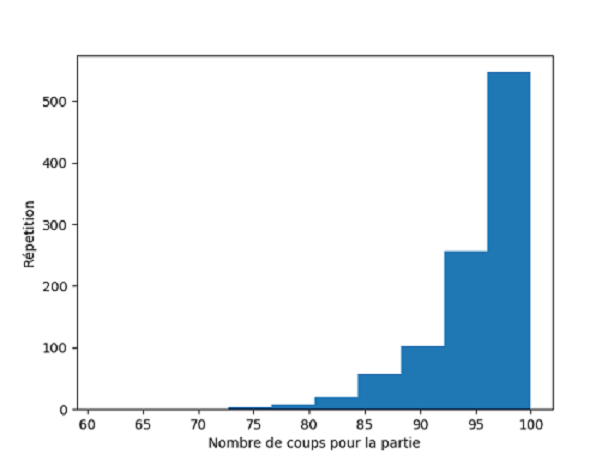
\includegraphics[]{Aleatoire.png}
    
    \subsection{Version heuristique}
    Dans cette méthode, on parcourt aléatoirement les cases jusqu'à trouver une case qui contient un bateau, alors on explore les cases adjacentes.
    Voici le graphique de distribution pour 1000 parties: \\
    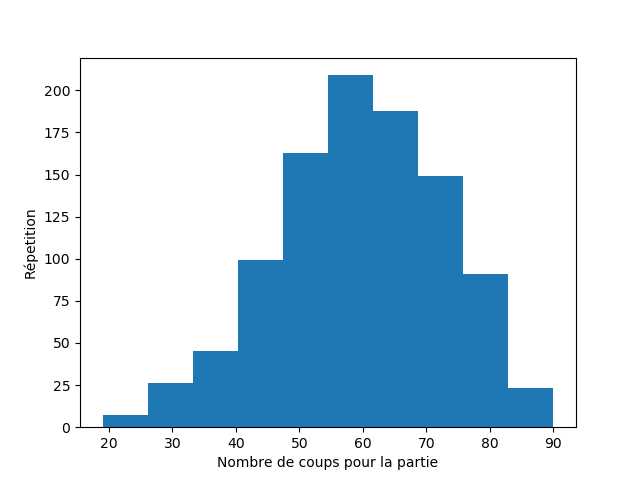
\includegraphics[width=\linewidth]{Heuristique.png}            
    Esperance expérimentale : 60 tours \\
    L'amelioration est bien apparente, car ici on s'aide du fait qu'une case a plus de chance de contenir un bateau si une case adjacente contient aussi un bateau.
    
    \subsection{Version probabiliste simplifiée}
    Dans cette méthode, on exploite le fait que l'on connaisse les cases déjà parcourue ainsi que les bateaux déjà coulés, on peut donc connaitre les positions qui contiennet probablement un bateau, ainsi que celles où c'est impossible.
    On procède de la manière suivante: à chaque tour, et pour chaque bateau restant, on parcourt toutes les cases non explorées, et on essaie de déposer le bateau sans prendre en compte les autres bateaux (car il existe beaucoup trop de dispositions possibles surtout vers le début), et si l'on parvient à le déposer, on augmente la probabilité que ces cases contiennent un bateau, et puis on chosit la case qui a la plus grande probabilité de contenir un bateau, et du coup, plus on a joué de coups, plus on est certain de connaitre les cases qui contiennent un bateau.
    Voici le graphique de distribution pour 1000 parties: \\
    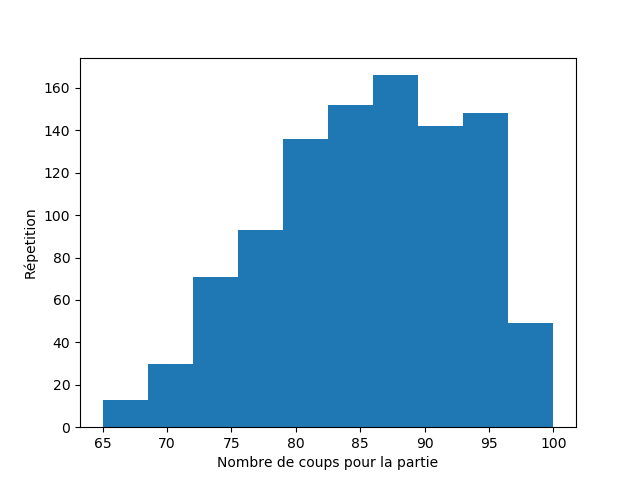
\includegraphics{Proba.png}            
    \\Esperance expérimentale : 85 tours \\
    Cette implementation est plus rapide que l'aléatoire, et si on la couple avec la méthode heuristique elle sera plus rapide que l'heuristique, je n'ai hélas pas réussi à coupler les 2 méthodes.

\section{Conclusion}
    Cette étude nous montre bien qu'une approche aléatoire peut fonctionner, mais est très lente et moins fiable par rapport à une approche stratégique bien étudiée (car certaines stratégies peuvent mêmes être pires qu'une aléatoire).
    \\Cette étude m'as aussi permis de remarquer que la nouvelle version 2008 du jeu (hexagonale) désavantage un des 2 joueurs, car il a moins de 25\% de disposition possibles par rapport à l'autre (17,290,404,311 VS 21,625,126,041).
    

% --------------------------------------------------------------
%     You don't have to mess with anything below this line.
% --------------------------------------------------------------
 
\end{document}